\titre{91-musy17}
\theme{equations}
\auteur{Nathan Scheinmann}
\niveau{1M}
\source{musy-2017}
\type{serie}
\piments{1}
\pts{}
\annee{2425}

\contenu{
	\tcblower
Sur le dessin ci-dessous, la figure ombrée est un carré, et le grand quadrilatère, un rectangle.

(Toutes les longueurs sont en cm.)

\hfill
\begin{minipage}[t]{0.5\textwidth}{
\vspace{0pt}
\begin{tikzpicture}
    \tkzDefPoint[label=below:{}](-1,-1){A}
    \tkzDefPoint[label=right:{}](-1,1){B}
    \tkzDefPoint[label=above:{}](2,0.5){C}
    \tkzDefPoint[label=above:{}](3,0.5){D}
    \tkzDefPoint[label=above:{}](2,-1){G}
    \tkzDefPoint[label=above:{}](3,1){E}
    \tkzDefPoint[label=above:{}](3,-1){F}

    \tkzDrawPolygon(A,B,E,F)
    \tkzDrawPolygon(F,G,C,D)
    \tkzFillPolygon[pattern=north west lines](F,G,C,D)
    \tkzDrawSegment[dashed,dim={$2$,15pt,right=2mm,midway,font=\footnotesize}](E,D)
    \tkzDrawSegment[dashed,dim={$x$,-15pt,right=2mm,midway,font=\footnotesize}](F,D)
    \tkzDrawSegment[dashed,dim={$6$,-15pt,below=2mm,midway,font=\footnotesize}](A,G)


\end{tikzpicture}
}
\end{minipage}
\begin{minipage}[t]{0.4\textwidth}{
\vspace{0pt}
Déterminer $x$ pour que l'aire de la partie blanche soit égale à $38 \mathrm{~cm}^2$.
}
\end{minipage}


}
\correction{
	\tcblower
	$\dfrac{13}{4}$
}

